\documentclass[a4paper,10.5pt]{article}
\usepackage[
  left=3cm, right=3cm, top=2.5cm, bottom=2.0cm,
  footskip=1.5cm, headheight=22.2pt, headsep=1cm,
  includehead, includefoot, heightrounded]{geometry}
\usepackage[utf8]{inputenc}
\usepackage[american]{babel}

%
\usepackage{csquotes}

% Creative commons icons
\usepackage{ccicons}


% Palatino for rm and math | Helvetica for ss | Courier for tt
%\usepackage{mathpazo} % math & rm
%\linespread{1.05}        % Palatino needs more leading (space between lines)
%\usepackage[scaled]{helvet} % ss
%\usepackage[varqu]{zi4} % tt

\usepackage{mathpazo} % math & rm
\usepackage{FiraSans}
\usepackage{FiraMono}
%\usepackage{sfmath}
%\usepackage{mathtools}
%\makeatletter
%\def\bfseries@sf{m}
%\SetSymbolFont{operators}{normal}{\math@encoding}{\math@sfdefault}{l}{n}
%\SetSymbolFont{operators}{bold}{\math@encoding}{\math@sfdefault}{m}{n}
%\DeclareSymbolFont{SFMath}{\math@encoding}{\math@sfdefault}{l}{sl}
%\SetSymbolFont{SFMath}{normal}{\math@encoding}{\math@sfdefault}{l}{sl}
%\SetSymbolFont{SFMath}{bold}{\math@encoding}{\math@sfdefault}{m}{\mathnormal@bold@shape}
%\makeatother


% Maths
% \usepackage{amsmath, amssymb, amsthm, mathtools}

% Graphics
\usepackage{graphicx}

% First page, bottom header
\usepackage[letterspace=150]{microtype}

% For the ifempty macro
\usepackage{etoolbox}

% For two columns bibliography
\usepackage{multicol}

% Sans-serif section titles
\usepackage{sectsty}
\allsectionsfont{\sffamily}

% Figure caption
\usepackage[labelsep=period]{caption}
\renewcommand{\captionfont}{\small}
\renewcommand{\captionlabelfont}{\small\sffamily\bfseries}


% Biber
\usepackage[
  backend=biber,
  style = numeric,
  % style=authoryear,
  sorting = none,
  giveninits = true,
  maxcitenames=3,
  mincitenames=1,
  maxbibnames=1000,
  isbn = false,
  url = false,
  doi = false,
  autocite = superscript,
  natbib = true]{biblatex}
\DeclareFieldFormat{labelnumberwidth}{#1\adddot}


% Hyperref & colors
\usepackage{xcolor}
\definecolor{blendedblue}{rgb}{0.2, 0.2, 0.6}
\definecolor{blendedred}{rgb}{0.8, 0.2, 0.2}
\usepackage[pdfusetitle,
            bookmarks=true,
            breaklinks=true,
            pdfborder={0 0 0},
            citecolor=blendedblue,
            colorlinks=true,
            linkcolor=blendedblue,
            urlcolor=blendedblue,
            citecolor=blendedblue,
            linktocpage=false,
            hyperindex=true,
            linkbordercolor=white]{hyperref}
\usepackage{hyperref}
\hypersetup{colorlinks=true}

% Author and affiliations
\usepackage{authblk}
\renewcommand\Affilfont{\normalfont\sf\footnotesize}
\renewcommand\Authfont{\sf\bfseries\small}

% Various convenient macros
\usepackage[many]{tcolorbox}
\newtcbox{\iconbox}[1][]{%
  enhanced,nobeforeafter,tcbox raise base, 
  boxrule=0.4pt, top=0pt, bottom=-1pt,
  right=1pt, left=1pt, arc=1pt, boxsep=1pt,
  fontupper={\tiny \sffamily}, before upper={\vphantom{dlg}},
  colframe=white, colback=black!10!white, coltext=black}
\newcommand{\orcid}[1]{\href{https://orcid.org/#1}{\iconbox{ID}}}
\newcommand{\doi}[1]{\href{http://doi.org/#1}{#1}}
\newcommand{\github}[1]{\href{https://github.com/#1}{github.com/#1}}
\definecolor{red}{HTML}{CF232B}
\newcommand{\ReScience}{{\bfseries Re\textcolor{red}{Science C}}}


% Line numbers (discrete color)
% \usepackage{lineno}
% \renewcommand{\linenumberfont}{\sf\footnotesize\color{lightgray}}


% Headers & footers
\usepackage{fancyhdr}
\pagestyle{fancy}
\fancyhf{}
\lhead{}
\renewcommand{\footrulewidth}{0.5pt}
\renewcommand{\headrulewidth}{0.0pt}

%\lhead{\footnotesize \sf ReScience~$|$
%                        \href{https://rescience.github.io}{rescience.github.io}}

% First page
\fancypagestyle{titlepage} {
  \fancyhf{}
  \chead{
   \sf \LARGE \ReScience\vspace{-5mm}\\
   \noindent\rule{9cm}{0.4pt}\\
   \normalsize \noindent \vspace{-3mm} \authorsSHORT~\articleYEAR
  }
  \renewcommand{\headrulewidth}{0.0pt}
  \renewcommand{\footrulewidth}{0.0pt}
  \cfoot{%\vfill \small \sf ReScience C\\
         \footnotesize {\lsstyle \normalfont \scshape \hspace{0.75pt} Open Access}
  }
}

% No date
\date{}




% =============================================================================
% DO NOT EDIT - automatically generated from metadata.yaml

\def \codeURL{https://github.com/ReScience/ReScience-template}
\def \codeDOI{10.5281/zenodo.27944}
\def \dataURL{}
\def \dataDOI{}
\def \editorNAME{Tiziano Zito}
\def \editorORCID{}
\def \reviewerINAME{Benoît Girard}
\def \reviewerIORCID{0000-0002-8117-7064}
\def \reviewerIINAME{Mehdi Khamassi}
\def \reviewerIIORCID{0000-0002-2515-1046}
\def \dateRECEIVED{09 June 2015}
\def \dateACCEPTED{12 August 2015}
\def \datePUBLISHED{14 August 2015}
\def \articleTITLE{ReScience Article Template}
\def \articleYEAR{2015}
\def \reviewURL{None}
\def \articleABSTRACT{This article is a proposition for a new article template for the ReScience C (computational replication) and ReScience X (experimental replication) journals. It is loosely based after Edward Tufte’s book style where the large left columns containes the main text and the right columns is used for auxiliary informations such as notes, captions or references. The template requires a standard TeXLive installation in order to compile it and this PDF has been compiled using TeXLive 2017 (pdflatex). Both the style, the layout and the colors of the template aim at giving ReScience a strong but subtle identity.}
\def \replicationBIB{M. Guthrie, A. Leblois, A. Garenne, and T. Boraud. Interaction between cognitive and motor cortico-basal ganglia loops during decision making: a computational study. In: Journal of Neurophysiology 109.12 (2013)}
\def \replicationDOI{10.1152/jn.00026.2013}
\def \contactNAME{Nicolas P. Rougier}
\def \contactEMAIL{Nicolas.Rougier@inria.fr}
\def \articleKEYWORDS{Latex, Template, ReScience}
\def \journalVOLUME{1}
\def \journalISSUE{1}
\def \articleNUMBER{1}
\def \articleDOI{}
\def \authorsFULL{Nicolas P. Rougier and Nicolas P. Rougier}
\def \authorsABBRV{N.P. Rougier and N.P. Rougier}
\def \authorsSHORT{Rougier and Rougier}
\title{\articleTITLE}
\date{}
\author[1,2,3,\orcid{0000-0002-6972-589X}]{Nicolas P. Rougier}
\affil[1]{INRIA Bordeaux Sud-Ouest, Bordeaux, France}
\affil[2]{LaBRI, Université de Bordeaux, Institut Polytechnique de Bordeaux, Centre National de la Recherche Scientifique, UMR 5800, Talence, France}
\affil[3]{Institut des Maladies Neurodégénératives, Université  de Bordeaux, Centre National de la Recherche Scientifique, UMR 5293, Bordeaux, France}

% =============================================================================


%\lfoot{\footnotesize \sf DOI:~\doi{\articleDOI}}
%\rhead{\footnotesize \sf \articleHEAD}
%\rfoot{\footnotesize \sf Volume \articleVOLUME~$|$~Article \#\articleNUMBER}
\lfoot{\footnotesize \sf ReScience C} %-- Vol. \journalVOLUME}
\rfoot{\footnotesize \sf \thepage}
%\rfoot{\\footnotesize \sf Volume \articleVOLUME~$|$~Article \#\articleNUMBER}
\rhead{\footnotesize \sf \authorsSHORT~\articleYEAR}
%\rfoot{\footnotesize \sf Volume \articleVOLUME~$|$~Article \#\articleNUMBER}



\title{\Large \sf \bfseries \articleTITLE}


\begin{document}
\maketitle
\thispagestyle{titlepage}
\noindent {\bfseries Abstract}. \articleABSTRACT\\

\noindent {\bfseries Keywords:} \articleKEYWORDS\\

\noindent {\bfseries A replication of }
          \href{http://doi.org/\replicationDOI}{\replicationBIB}\\

% =============================================================================
\begin{tikzpicture}[remember picture, overlay]
  \node [shift={(+1.5cm,-4cm)}] at (current page.north west) {
     \begin{tikzpicture}[remember picture, overlay]
       \fill [fill=red, opacity=1.0] (0,0) rectangle (2.cm,4cm);
       \node [shift={(1cm,1cm)}, opacity=1.0]
             {
\includegraphics[width=1.5cm]{logo.pdf}};
     \end{tikzpicture}
  };
\end{tikzpicture}

%% \begin{tikzpicture}[remember picture, overlay]
%%   \node [shift={(+0cm,-2.5cm)}] at (current page.north west) {
%%      \begin{tikzpicture}[remember picture, overlay]
%%        \fill [fill=red, opacity=1.0] (0,0) rectangle (2.5cm,2.5cm);
%%        \node [shift={(1.25cm,1.5cm)}, opacity=1.0]
%%              {
\includegraphics[width=1.5cm]{logo.pdf}};
%%        \node [color=white, shift={(1.25cm,.4cm)}]
%%              {\footnotesize \sffamily \scshape \bfseries ReScience C};
%%      \end{tikzpicture}
%%   };
%% \end{tikzpicture}


\vfill
\noindent\makebox[\textwidth]{\rule{\textwidth}{0.4pt}}
{\footnotesize \sf
  \noindent \textbf{Cite as}: \articleTITLE, \authorsABBRV.
                              In: {\em ReScience C}
                              \journalVOLUME(\#\articleNUMBER), \articleYEAR.
                              \textbf{DOI} \doi{\articleDOI}.\par
~\\
\noindent \textbf{Code repository} at \href{https://\codeURL}{\codeURL} --
          \textbf{DOI}                \doi{\codeDOI}\\
\ifdefempty{\dataURL}{}{
\noindent \textbf{Data repository} at \href{https://\dataURL}{\dataURL} --
          \textbf{DOI}                \doi{\dataDOI}\\
}
~\\
\noindent \textbf{Edited by}   \editorNAME$^{\orcid{\editorORCID}}$ --
          \textbf{Reviewed by} \reviewerINAME$^{\orcid{\reviewerIORCID}}$ 
           \&                  \reviewerIINAME$^{\orcid{\reviewerIIORCID}}$ --
                               \href{\reviewURL}{Open Review}\par
\noindent \textbf{Received}  \dateRECEIVED~--
          \textbf{Accepted}  \dateACCEPTED~--
          \textbf{Published} \datePUBLISHED\par
\noindent \textbf{Copyright} ©~\articleYEAR~\authorsABBRV\par
\noindent \textbf{Published} under a Creative Commons Attribution 4.0 International
          (\href{https://creativecommons.org/licenses/by/4.0/}{\ccLogo\ccAttribution})
          license\par
~\\
\noindent \textbf{Corresponding author}:
\contactNAME~(\href{mailto:\contactEMAIL}{\contactEMAIL})\\
\noindent \textbf{Competing Interests}:
           The authors have declared that no competing interests exist\par
}
\clearpage

%=============================================================================

\newgeometry{
  left=2cm, right=6cm, top=1.0cm, bottom=1.5cm,
  marginpar=4cm,
  footskip=1.5cm, headsep=1cm, includehead, includefoot, heightrounded}


%=============================================================================
\section*{Introduction}

What a nice template\footnote{I did it myself!} for \citep{Rougier:2017}
\marginpar{\sf \footnotesize Margin note can be used to insert a message in the
  margin such as for example a reference: \fullcite{Rougier:2017}}. \lipsum*[1]


\subsection*{Figures}

\begin{figure}[htbp]
   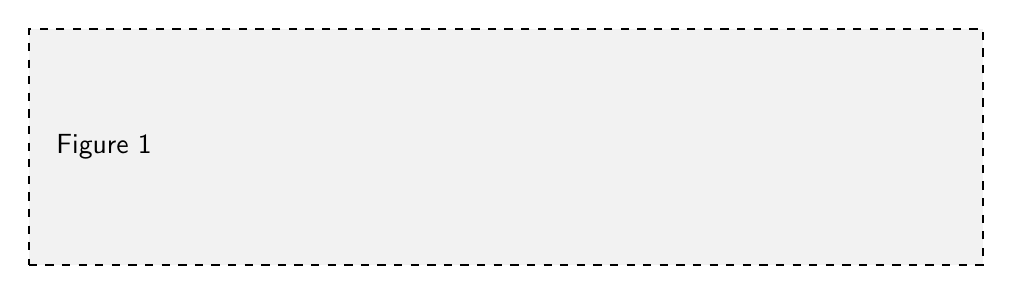
\begin{tikzpicture}
     \node[draw, fill=black!5, dashed, thick,
       text width=.98\textwidth, minimum height=3cm] at (0,0) {~~\sf Figure 1};
   \end{tikzpicture}
    \captionof{figure}{Figure caption.}
    \label{fig:1}
\end{figure}

\subsection*{Tables}
\begin{table}[htbp]
\begin{minipage}{.45\textwidth}
  \begin{tabularx}{\textwidth}{|XX|}
      \hline
      \bfseries Header 1 & \bfseries Header 2\\
      \hline
      Item 1 & Item 2\\
      Item 1 & Item 2\\
      Item 1 & Item 2\\
      \hline
    \end{tabularx}
    \captionof{table}{Table caption.}
    \label{tab:1}
\end{minipage}
\hfill
\begin{minipage}{.45\textwidth}
  \begin{tabularx}{\textwidth}{|XX|}
      \hline
      \bfseries Header 1 & \bfseries Header 2\\
      \hline
      Item 1 & Item 2\\
      Item 1 & Item 2\\
      Item 1 & Item 2\\
      \hline
    \end{tabularx}
    \captionof{table}{Table caption.}
    \label{tab:2}
\end{minipage}
\end{table}

\subsection*{Equations}
The well known Pythagorean theorem \(x^2 + y^2 = z^2\) was proved to be invalid
for other exponents.  Meaning equation \eqref{eq:1} has no integer solutions:
%%
\begin{equation}
  \label{eq:1}
  x^n + y^n = z^n
\end{equation}
\marginpar{\sf \footnotesize
           \vspace{-4em} I have a proof but it doesn't fit in the margin...}


\subsection*{Listings}
\begin{lstlisting}[language=python,
                   caption={Listing caption.},
                   label={lst:1}]
# Standard import
import this

text = "Some text"
\end{lstlisting}


\section*{Conclusion}

This is a short article.\\

\lipsum*[2]\\

%=============================================================================


\renewcommand*{\bibfont}{\footnotesize \sffamily}
\begingroup\setlength{\multicolsep}{0pt}
\begin{multicols}{2}[\printbibheading]
\printbibliography[heading=none]
\end{multicols}\endgroup
% \printbibliography[title=References]

\end{document}

